\section{Interaction}
\label{sec:scope_interaction}

In this section we describe how a user, or a program, should be able
to interact with the \textsc{TraceDroid} framework in order to obtain traces of a
running app. First the Android SDK needs to be installed on the
machine where we want to run the sandbox. After installation an
Android Virtual Device (AVD) has to be created: it will work as a
container with all the properties necessary for an Android system
image, in this case the custom \textsc{TraceDroid} one, to be emulated. We can
then start the emulator and interact with the modified Android sandbox
via the \texttt{adb} (Android Debug Bridge) command line interface.

Figure~\ref{fig:scope_interaction} shows how to interact with the system. The actor is
depicted as a user but it can also be automated in order to plug the
custom image into a bigger framework like \textsc{TAP}. After starting the
emulator the user interacts with the system with the command line
interface provided by the adb tool. In the case we want to trace an
app that is not installed in the AVD we first need to install it with
adb. This is not shown in the sequence diagram for simplicity.

The user, or the program that uses the dynamic analysis sandbox,
first locates the unique identifier (\texttt{uid}) of the application to
be profiled, then writes it to a file. This file, named uid, is afterwards pushed to the
AVD \texttt{/sdcard/} via adb. The actor, after this, chooses between the
activities that the application offers and starts one of them. All the
activities should be started in order to have more comprehensive and
detailed dynamic analysis of the process, this is exactly what \textsc{TAP}
does. The activity is then started by sending the command to \texttt{adb}.

The system, at this point, gathers control and adb sends the app's activity
invocation to the \textit{Activity Manager}. The AM, a process-like
manager, forwards the intent of starting a new activity to the \emph{Zygote}
process. The \emph{Zygote}, the parent of all the VM, invokes a \texttt{fork()} system
call to create a new virtual machine that performs as a container of
the application whose activity is started. The functions in the \texttt{Init} file create a new VM. These functions are modified in the \textsc{TraceDroid} version
in order to check whether the uid of the process started is the same as the
one stored in \texttt{/sdcard/uid}. Depending on whether the uid is the same or
not we have two different flows:
\begin{enumerate*}
  \item The uid is the same: the activity is started and the modified \texttt{Profile} class is activated to filter all the calls made by the process. The traces are then written to files under \texttt{/sdcard/}. When the activity finishes the VM returns, without killing the process, and the user can pull the dynamic analysis results from the \texttt{/sdcard/} via \texttt{adb}. 
  \item The uid is not the same: the activity is started but the \texttt{Profile} class is not activated since the user did not specify to trace this process. In this case the new VM completes the requested activity and returns to the AM once it has finished. 
\end{enumerate*}

This design respects the requirements points specified in the previous
section. The described sequence provides both a common interface for
tracing an app (the push uid \texttt{/sdcard/}) and for obtaining the dynamic
analysis results (the pull \texttt{/sdcard/traces*}). The system, furthermore,
allows for full automation using the \texttt{adb} command line tool.

\begin{figure}[!h]
    \centering
    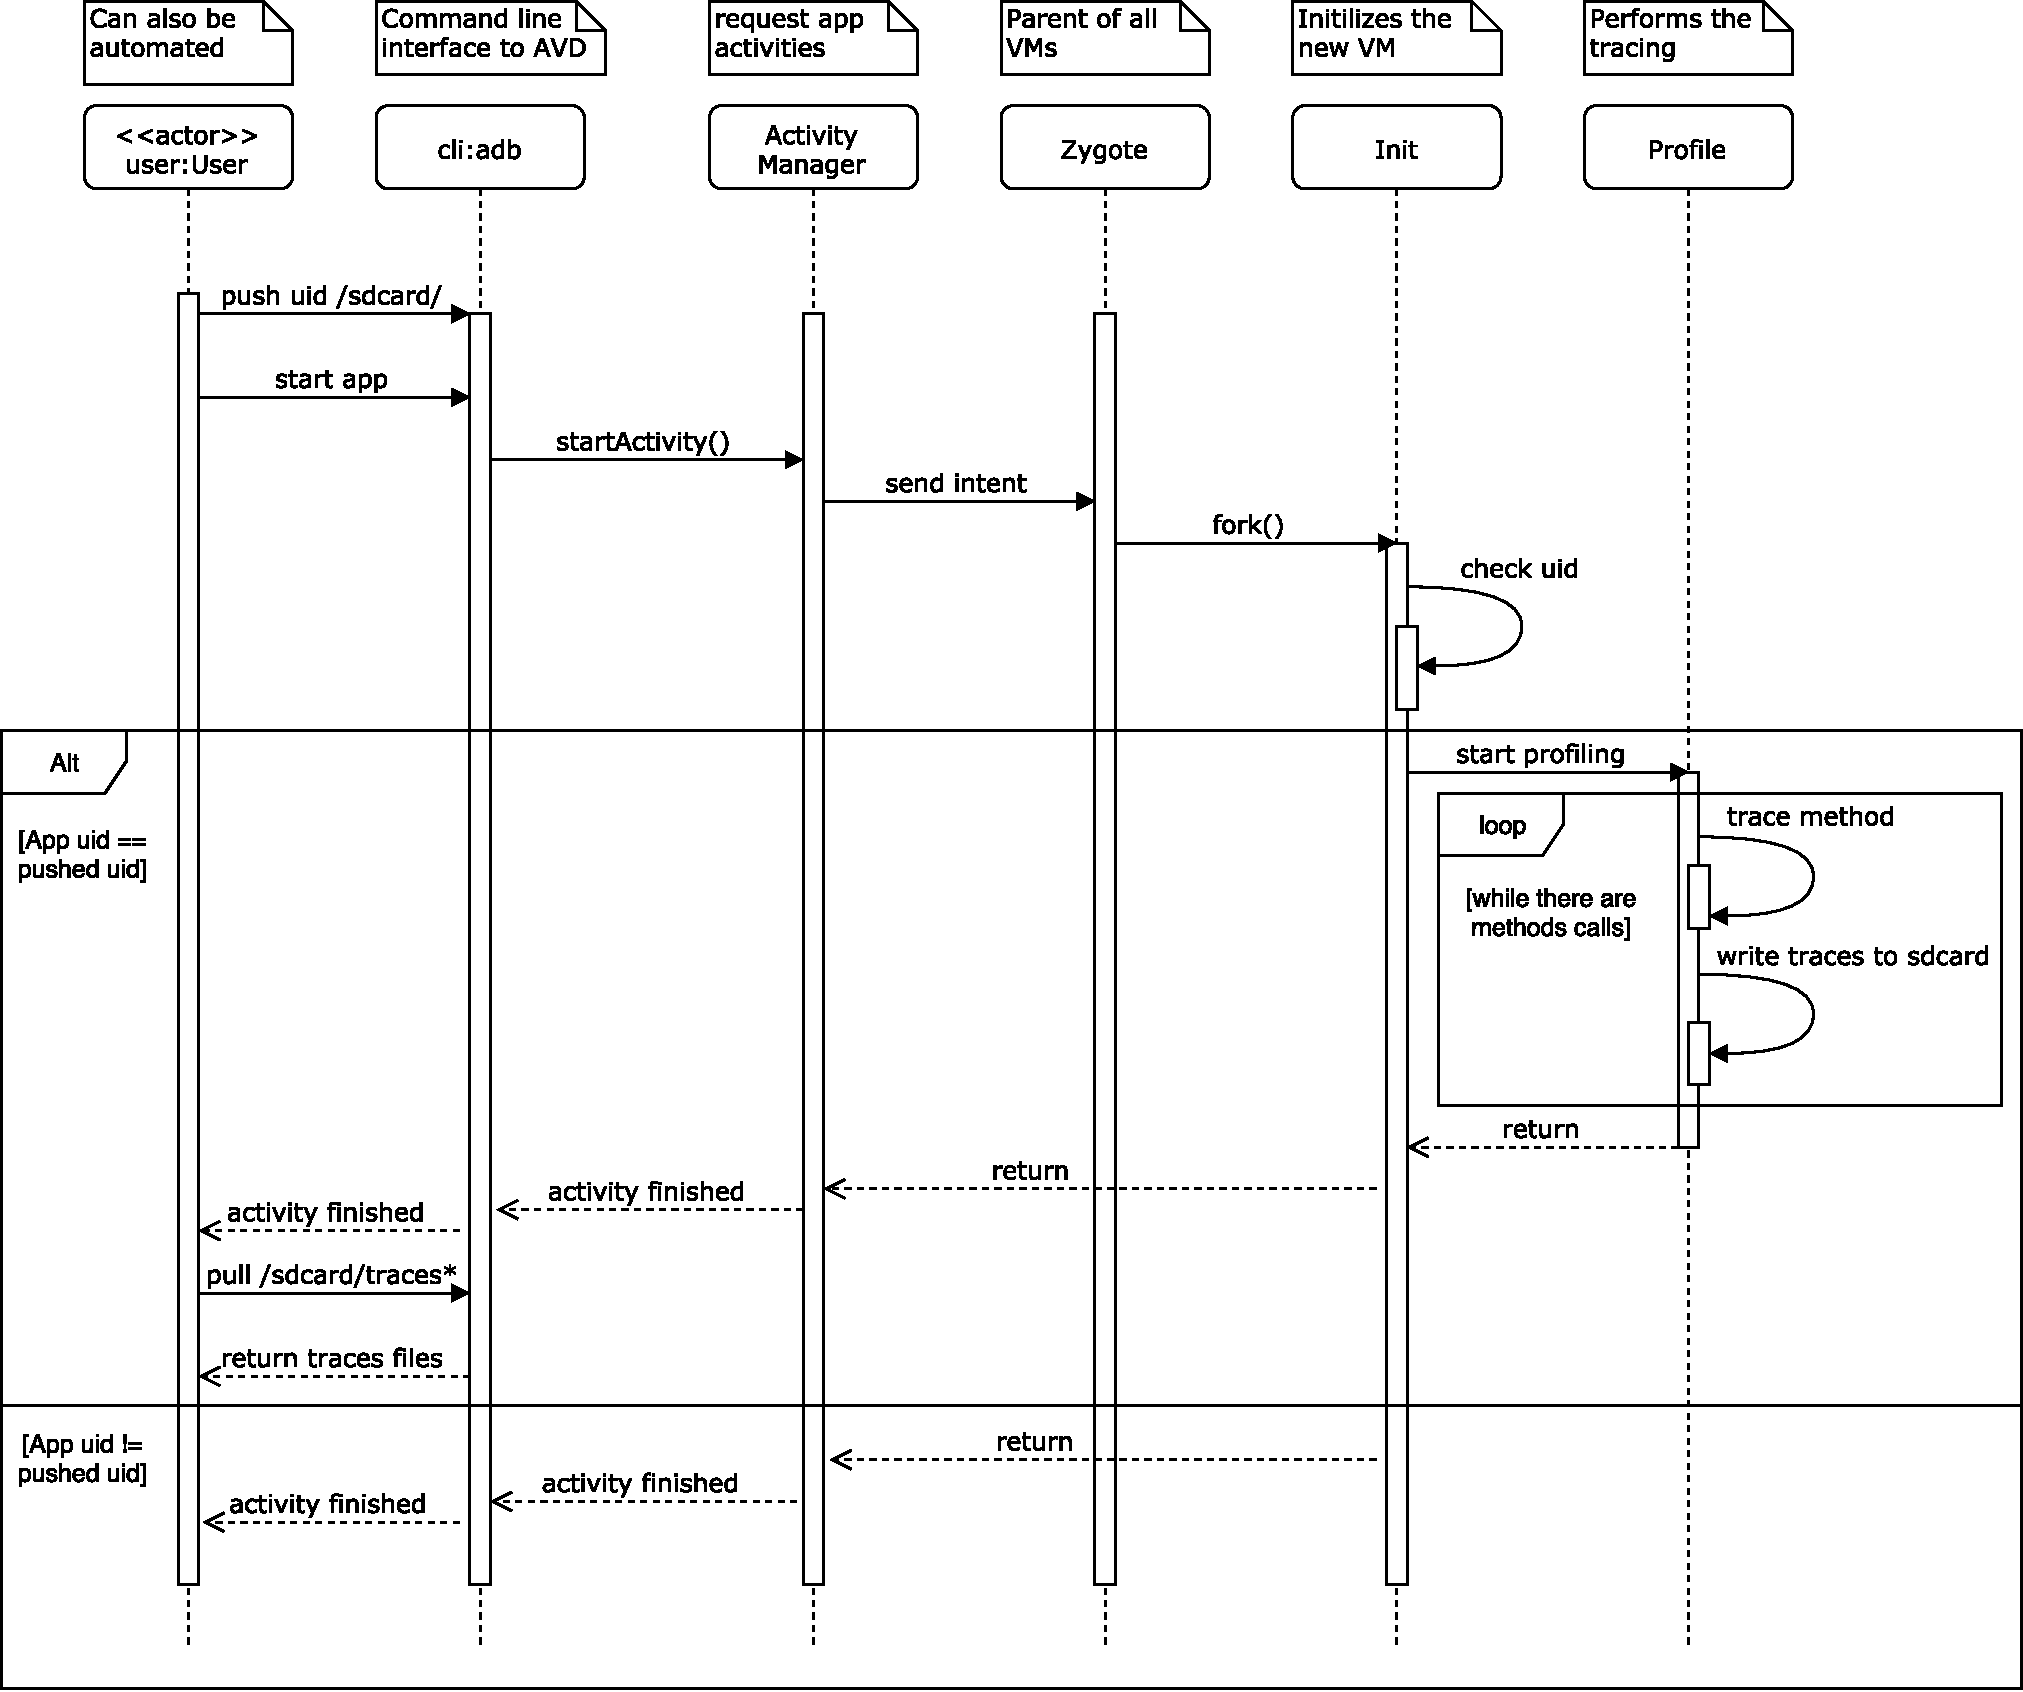
\includegraphics[width=15cm]{./img/design/interaction.pdf}
    \caption{Interaction Sequence Diagram}
    \label{fig:scope_interaction}
\end{figure}
